\chapter{Interactions}

Lorsque la lumière traverse un milieu participant, de multiples interactions peuvent avoir lieu au fur et à mesure que le rayon de lumière avance dans le milieu et rencontre des particules. La fréquence et la puissance de ces interactions vont dépendre de plusieurs propriétés du milieu participant, comme la densité par exemple. Ces propriétés varient dans le milieu, celui-ci étant rarement globalement homogène. Lorsque nous en seront à l'algorithme, il sera donc possible de décomposer le milieu en une grille 3D de fragments homogènes où les propriétés du milieu seront constantes.

\section{Absorption}

Lorsque la lumière arrive sur une particule, celle-ci fait obstruction et un certains nombres de photons ne parviennent donc pas à continuer leur chemin, c'est l'\textbf{absorption} (Figure \ref{fig:absorption}).

\begin{figure}[h!]\label{fig:absorption}
\centering
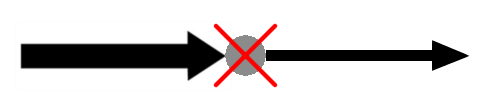
\includegraphics[width=100mm]{particule_absorption.png}
\caption{Absorption par une particule}
\end{figure}

Un milieu participant homogène possède un \textit{coefficient d'absorption} $\sigma_{a}$ qui correspond à la probabilité que la lumière soit absorbée lors de son passage dans le milieu. Une estimation simple et constante de ce coefficient est la suivante :
\large
$$\sigma_{a}(p, \omega) = \pi r^{2} N,$$
\normalsize
où $r$ est le rayon des particules (m) et $N$ la densité des particules (m$^{-3}$). $\sigma_{a}$ est donc en m$^{-1}$.

La valeur qui nous intéresse est la variation de radiance entre le faisceau arrivant sur la particule et celui en partant. Cette différence ne dépend que de la radiance initiale et du coefficient d'absorption du milieu traversé :
\large
\begin{equation}
    \Delta L(p, \omega) = L_{o}(p, \omega) - L_{i}(p, \omega) = -\sigma_{a}(p, \omega)L_{i}(p, \omega)dt
.\end{equation}
\normalsize

\section{Out-Scattering}

Lorsque le faisceau de lumière rencontre une particule dans le milieu, les photons qui le composent peuvent être absorbés (cf. Absorption) mais également renvoyés dans d'autres directions. C'est ce qu'on appelle l'\textbf{out-scattering} (figure \ref{fig:out_scattering}).

\begin{figure}[h!]\label{fig:out_scattering}
\centering
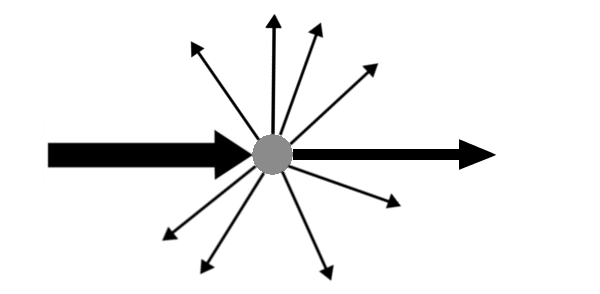
\includegraphics[width=100mm]{particule_out_scattering.png}
\caption{Out-scattering causé par une particule}
\end{figure}

Tout comme il existe un coefficient d'absorption, le milieu possède un \textit{coefficient de dispersion} $\sigma_{s}$ correspondant à la probabilité que le faisceau de lumière soit dispersé.

Son impact est semblable au coefficient d'absorption :
\large \begin{equation}
    \Delta L(p, \omega) = -\sigma_{s}(p, \omega)L_{i}(p, \omega)dt
.\end{equation} \normalsize

\section{Extinction}

Nous avons deux interactions qui atténuent la lumière lorsque celle-ci passe dans un milieu participant : l'absorption et l'out-scattering. Ces deux effets combinés donnent l'\textbf{extinction}. Un milieu participant homogène possède donc, de manière analogue aux deux interactions vues précédemment, un \textit{coefficient d'atténuation}, ou \textit{coefficient d'extinction} $\sigma_{t}$. Celui-ci est tout simplement donné par :
\large
$$\sigma_{t} = \sigma_{a} + \sigma_{s}.$$
\normalsize
Ce qui conduit à :
\large \begin{equation}
    \Delta L(p, \omega) = -\sigma_{t}(p, \omega)L_{i}(p, \omega)dt
.\end{equation} \normalsize \newline\par

Nous pouvons maintenant calculer non pas un delta de radiance mais une \textbf{proportion}. Soient $p$ et $p'$ deux points sur un rayon de direction normalisée $\omega$, à une distante $d$ l'un de l'autre. Alors nous avons :
\large \begin{equation} \label{eq:transmittance_definition}
    T_{r}(p\longrightarrow p') = e^{-\int_{0}^{d} \sigma_{t}(p+t\omega, \omega)dt} = e^{-\tau}
.\end{equation} \normalsize
où $T_{r}$ est la \textit{transmittance}, la proportion de radiance qui est transmise de $p$ à $p'$ sur un rayon traversant le milieu participant. $\tau$ est appelé l'\textit{épaisseur optique} du milieu. Sachant que dans un milieu homogène $\sigma_{t}$ est constant, on a $T_{r}(p\longrightarrow p') = e^{-\sigma_{t}d}$ : c'est la \textit{loi de Beer}.\par
Ainsi, soit $L_{o}(p, \omega)$ la radiance sortant d'un point $p$ d'une surface dans une direction normalisée $\omega$. Ce rayon traverse une milieu participant et arrive sur un autre point $p'$. Alors la radiance incidente à ce point $p'$ est donnée par (cf. figure \ref{fig:transmittance}) :
\large \begin{equation}
    L_{i}(p', -\omega) = T_{r}(p\longrightarrow p')L_{o}(p, \omega)
.\end{equation} \normalsize \par

Il va donc de soit que dans le vide, $T_{r}(p\longrightarrow p') = 1$.

\begin{figure}[h!]\label{fig:transmittance}
\centering
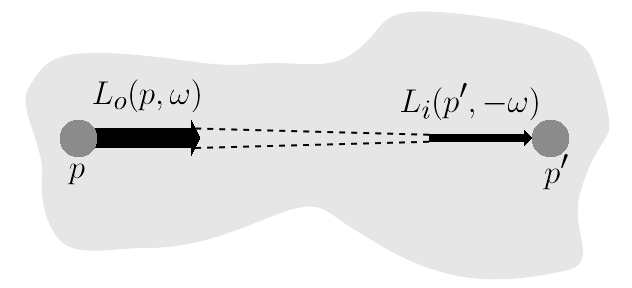
\includegraphics[width=100mm]{transmittance.png}
\caption{Atténuation d'un rayon grâce à la transmittance}
\end{figure}

Une propriété importante de la transmittance, qui nous sera utile pour l'écriture de l'algorithme, dit que la transmittance est multiplicative le long des points sur un rayon. Soient $p$ et $p''$ deux points sur un rayon. Et soit $p'$ un point entre $p$ et $p''$. Alors on a :
\large \begin{equation}
    T_{r}(p\longrightarrow p'') = T_{r}(p\longrightarrow p')T_{r}(p'\longrightarrow p'')
.\end{equation} \normalsize

\section{Émission}

Lors de son passage dans un milieu participant, la radiance du rayon ne fait pas que diminuer. Certains milieux participants peuvent auto émettre de la lumière. C'est ce qu'on appelle l'\textbf{émission} (figure \ref{fig:emission}). Lorsque le faisceau de lumière passe sur une particule émettant de la lumière, celui-ci gagne en intensité.

\begin{figure}[h!]\label{fig:emission}
\centering
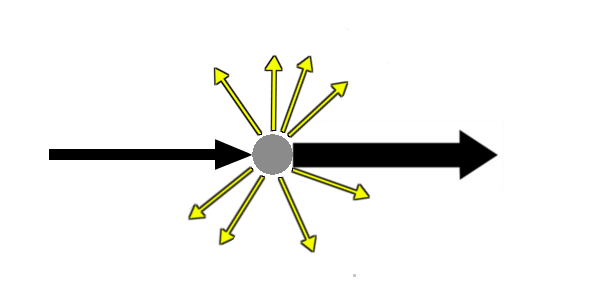
\includegraphics[width=100mm]{particule_emission.png}
\caption{Émission d'une particule}
\end{figure}

La lumière émise, qui ne dépend ici pas du rayon incident au point $p$ s'ajoute à la radiance :
\large \begin{equation}
    \Delta L(p, \omega) = L_{ve}(p, \omega)
.\end{equation} \normalsize

\section{In-Scattering}

Nous avons vu que lors d'une dispersion de la lumière (out-scattering), des photons étaient déviés de leur trajectoire, ne contribuant donc plus à la radiance du rayon initialement lancé. Ces photons ne disparaissent cependant pas et vont contribuer ailleurs, ils vont s'ajouter à un autre rayon avec qui ils partagent la trajectoire. Cela dit, il serait lourd de calculer, à chaque point p et chaque évènement d'out-scattering, les contributions de chaque nouveau rayon de contributions individuellement faibles. Pour simuler cet effet, nous avons donc l'interaction \textbf{in-scattering}(figure \ref{fig:in_scattering}).\par
Lorsque le faisceau rencontre une particule et que nous voulons calculer les contributions de chacune des interactions présentées précédemment, nous ajoutons la contribution des ces radiances perdues.

\begin{figure}[h!]\label{fig:in_scattering}
\centering
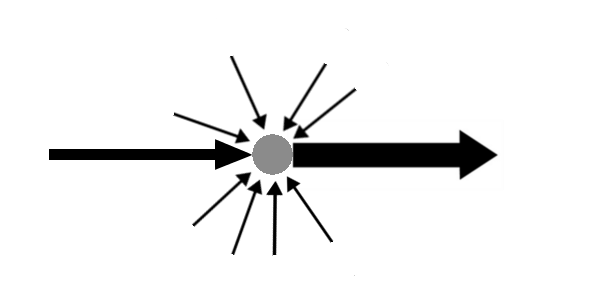
\includegraphics[width=100mm]{particule_in_scattering.png}
\caption{In-scattering sur une particule}
\end{figure}

Cet ajout dépend naturellement du \textit{coefficient de dispersion} $\sigma_{s}$, puisque l'\textit{out-scattering} et l'\textit{in-scattering} sont dûs à la même réaction.\par

Le calcul de cett interaction est cependant un peu plus complexe. En effet, là où pour l'out-scattering nous n'avions pas besoin de savoir ce qu'il se passait de la radiance perdue, nous devons ici prendre en compte que nouveaux rayons qui ont voyagé dans le milieu avant d'arriver jusqu'à notre particule, et dont ma direction a changé. C'est ici que nous utilisons la \textbf{fonction de phase} $\rho$ de notre milieu :
\large \begin{equation}
  \Delta L(p, \omega) = \sigma_{s}(p, \omega) \int_{\Omega4\pi}\rho(p, -\omega'\longrightarrow\omega)d\omega' dt  
.\end{equation} \normalsize \par

Le domaine d'intégration est ici la sphère complète autour du point $p$. Puisque nous ne sommes pas sur une surface, il n'y a en effet pas d'obstruction faite ne laissant qu'une hémisphère de possibilités.

\section{Source}

Au final, nous avons deux interactions qui viennent augmenter la radiance d'un rayon lors de son passage dans un milieu participant : l'émission et l'in-scattering. Cela nous donne la \textbf{source} $L_s$ de radiance qui va venir s'ajouter à la radiance initiale :
\large \begin{equation}\label{eq:source}
    L_s(p, \omega) = L_{ve}(p, \omega) + \sigma_{s}(p, \omega) \int_{\Omega4\pi}\rho(p, -\omega'\longrightarrow\omega)L_i(p, \omega')d\omega'
.\end{equation} \normalsize
En découle :
\large \begin{equation}
    \Delta L(p, \omega) = L_s(p, \omega)dt
.\end{equation} \normalsize